\documentclass[10pt]{exam}
\usepackage[hon]{template-for-exam}
\usepackage{tikz}
\usetikzlibrary{shadings,decorations.pathmorphing,arrows.meta,patterns}


\title{Torque Lab}
\author{Rohrbach}
\date{\today}

\begin{document}
\maketitle

\noindent
An object is in \emph{static equilibrium} when it is not rotating or translating.  This means it has no net force ($\Sigma F=ma$) or net torque ($\Sigma \tau =0$).  The goal of this lab take a closer look at a simple case of static equilibrium and see how torques can cancel in equilibrium conditions.

\begin{questions}
  \begin{EnvUplevel}
    \section*{Situation A}

    In a moment, we will set up the meter stick to look like this: 

  \end{EnvUplevel}

  \begin{EnvUplevel}
    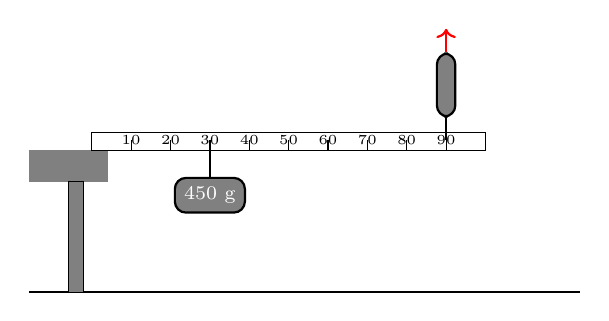
\begin{tikzpicture}
      \def\meter{5}
      \draw[thick] (0,0) -- (7,0);
      \draw (0,1.8)
        -- ++ (1,0)
        -- ++ (0,-.4)
        -- ++ (-1,0);
      \fill[gray] (0,1.8) rectangle ++(1,-.4);
      \draw[fill=gray] (0.5,0) rectangle (0.7,1.4);
      \draw (0.8,1.8) coordinate (0) 
        rectangle ++(\meter,0.23);
      \foreach \i in {10,20,30,40,50,60,70,80,90} {
        \draw (0) ++(\i*\meter/100,0) -- ++(0,0.13) 
          node[font=\tiny] (\i) {\i};
      }

      \draw[thick] (30.center) -- ++(0,-0.7)
        node[fill=gray, rounded corners, draw=black, text=white, font=\scriptsize] {450 g};

      \draw[thick] (90.center) -- ++(0,0.7)
        node[fill=gray, rounded corners, draw=black, text=white, minimum height=0.8cm] (scale) {};
      
      \draw[red,thick, ->] 
        (scale.north) -- ++(0,0.3);

    \end{tikzpicture}

  \end{EnvUplevel}
    


  \question
    Find the mass of the meter stick.
    \vs

  \question
    What is the lever arm of this mass?  (Think about {\sc CM})
    \vs
  
  \question
  	How many torques are acting on this system?  Draw them each on the diagram.  Write down the forces and lever arms ($r$) of each torque below.  Think about whether each torque is positive or negative.

  \question
	  Set up your equilibrium equation $\Sigma\tau=0$.  Solve for the force that your scale should read.
    \vs[5]

  \question
	  Your answer is your expected reading for the two scale.  Now set up the experiment and see how close your readings are to the expected values.

    \begin{tabular}{*{3}{|p{12em}}|}
      \hline
      Expected & Measured & Percent Error \\
      \hline
      && \\[2em]
      \hline
    \end{tabular}

  \pagebreak
  \begin{EnvUplevel}
    \section*{Situation B}

    In a moment, we will set up the meter stick to look like this:
  \end{EnvUplevel}

  \begin{EnvUplevel}
    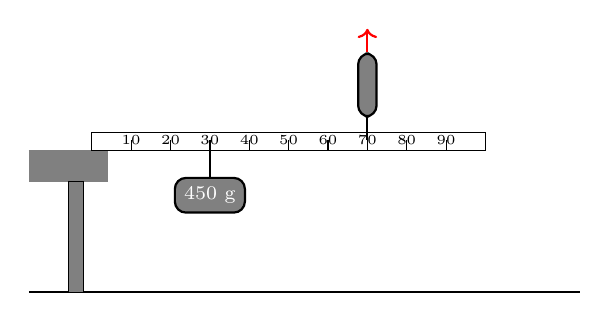
\begin{tikzpicture}
      \def\meter{5}
      \draw[thick] (0,0) -- (7,0);
      \draw (0,1.8)
        -- ++ (1,0)
        -- ++ (0,-.4)
        -- ++ (-1,0);
      \fill[gray] (0,1.8) rectangle ++(1,-.4);
      \draw[fill=gray] (0.5,0) rectangle (0.7,1.4);
      \draw (0.8,1.8) coordinate (0) 
        rectangle ++(\meter,0.23);
      \foreach \i in {10,20,30,40,50,60,70,80,90} {
        \draw (0) ++(\i*\meter/100,0) -- ++(0,0.13) 
          node[font=\tiny] (\i) {\i};
      }

      \draw[thick] (30.center) -- ++(0,-0.7)
        node[fill=gray, rounded corners, draw=black, text=white, font=\scriptsize] {450 g};

      \draw[thick] (70.center) -- ++(0,0.7)
        node[fill=gray, rounded corners, draw=black, text=white, minimum height=0.8cm] (scale) {};
      
      \draw[red,thick, ->] 
        (scale.north) -- ++(0,0.3);

    \end{tikzpicture}

  \end{EnvUplevel}

  \question
	  Show all work for calculating the reading of the scale:

    \question
	  Your answer is your expected reading for the two scale.  Now set up the experiment and see how close your readings are to the expected values.

    \begin{tabular}{*{3}{|p{12em}}|}
      \hline
      Expected & Measured & Percent Error \\
      \hline
      && \\[2em]
      \hline
    \end{tabular}


  
\end{questions}

\end{document}